\documentclass[aspectratio=169,12pt,t]{beamer}

% --- Theme: Metropolis (modern, clean) ---
\usetheme[progressbar=frametitle,numbering=fraction,block=fill]{metropolis}

% --- Fira Sans font (install texlive-fonts-extra if missing) ---
\IfFileExists{FiraSans.sty}{\usepackage[sfdefault]{FiraSans}}{}

% --- Light background with warm accent ---
\definecolor{mDarkTeal}{RGB}{35,55,59}
\definecolor{mLightBrown}{RGB}{235,228,216}
\definecolor{mAccent}{RGB}{140,70,20}

\setbeamercolor{normal text}{fg=mDarkTeal,bg=white}
\setbeamercolor{alerted text}{fg=mAccent}
\setbeamercolor{frametitle}{bg=mDarkTeal,fg=white}
\setbeamercolor{progress bar}{fg=mAccent,bg=mLightBrown}
\setbeamercolor{title separator}{fg=mAccent}
\setbeamercolor{progress bar in head/foot}{fg=mAccent,bg=mLightBrown}
\setbeamercolor{progress bar in section page}{fg=mAccent,bg=mLightBrown}

% --- Packages ---
\usepackage[utf8]{inputenc}
\usepackage{amsmath,amssymb,amsthm}
\usepackage{mathrsfs}
\usepackage{tikz}
\usetikzlibrary{arrows.meta,positioning,calc,decorations.pathreplacing,shapes,patterns}
\usetikzlibrary{shadows.blur,backgrounds,fadings}
\usepackage{pgfplots}
\pgfplotsset{compat=1.18}

% --- Shared diagram styling (consistent, polished look across all figures) ---
\tikzset{
  % organic, soft-shadowed "set" blobs
  setblob/.style={line width=1pt, rounded corners,
    blur shadow={shadow blur steps=8, shadow opacity=22,
                 shadow xshift=0pt, shadow yshift=-1.4pt}},
  blobblue/.style={setblob, draw=defcolor, fill=defcolor!10},
  blobred/.style={setblob, draw=thmcolor, fill=thmcolor!10},
  blobamber/.style={setblob, draw=excolor, fill=excolor!12},
  % the mapping arrow f
  mapf/.style={-{Stealth[length=3mm,width=2.4mm]}, line width=1.2pt, mAccent},
  % clean axes
  axisln/.style={-{Stealth[length=2.6mm]}, line width=0.8pt, gray!75},
  % graphed curves
  curveln/.style={line width=1.5pt, line cap=round, line join=round},
  % light projection / helper lines
  projln/.style={dash pattern=on 2.6pt off 2pt, line width=0.7pt},
}
% point marker with a white halo: \dotpt{color}{(coord)}
\newcommand{\dotpt}[2]{%
  \fill[white] #2 circle (3.4pt);
  \fill[#1] #2 circle (2.2pt);
}
% reusable organic blob outlines at the origin (~3.0 x 2.0), use inside a scope
% \blobpath : the source set E
\def\blobpath{plot[smooth cycle, tension=0.85] coordinates
  {(-1.5,0.05) (-1.12,0.82) (-0.05,1.05) (1.08,0.86) (1.56,0.08)
   (1.18,-0.82) (0.05,-1.06) (-1.2,-0.72)}}
% \blobpathdef : a deformed image, distinctly different shape (f need not be rigid)
\def\blobpathdef{plot[smooth cycle, tension=0.9] coordinates
  {(-1.45,-0.2) (-1.35,0.7) (-0.55,1.18) (0.45,0.78) (1.5,0.95)
   (1.62,-0.05) (0.95,-0.92) (-0.15,-0.78) (-0.95,-1.05)}}

% --- Semi-transparent white highlight for text on top of background images ---
\usepackage[most]{tcolorbox}

% Inline highlight: \hl{short text}
\newtcbox{\hl}{%
  nobeforeafter, tcbox raise base,
  colback=white, opacityback=0.6,
  colframe=white, opacityframe=0,
  sharp corners, boxsep=2pt, left=3pt, right=3pt, top=2pt, bottom=2pt%
}

% Block highlight: \begin{hlbox} ... \end{hlbox}  (multi-line, paragraphs, itemize)
% Optional argument accepts any tcolorbox key, e.g. [width=0.6\linewidth]
\newtcolorbox{hlbox}[1][]{%
  enhanced, breakable,
  colback=white, opacityback=0.6,
  colframe=white, opacityframe=0,
  boxsep=3pt, left=6pt, right=6pt, top=4pt, bottom=4pt,
  sharp corners,
  {#1}%
}

% --- Custom colors for content types ---
\definecolor{defcolor}{RGB}{25,85,120}
\definecolor{thmcolor}{RGB}{140,35,35}
\definecolor{proofcolor}{RGB}{35,100,50}
\definecolor{excolor}{RGB}{140,75,10}
\definecolor{remcolor}{RGB}{90,90,90}

% --- Beamer blocks for mathematical content types (semi-transparent) ---
\tcbset{hlblockbase/.style={
  enhanced, breakable,
  coltitle=white, fonttitle=\bfseries,
  opacitybacktitle=0.8, opacityback=0.6,
  opacityframe=0,
  sharp corners,
  boxsep=1pt, left=5pt, right=5pt, top=2pt, bottom=2pt,
  toptitle=1pt, bottomtitle=1pt
}}

\newtcolorbox{defblock}[1]{hlblockbase, title={#1},
  colbacktitle=defcolor, colback=defcolor!15, colframe=defcolor}
\newtcolorbox{thmblock}[1]{hlblockbase, title={#1},
  colbacktitle=thmcolor, colback=thmcolor!15, colframe=thmcolor}
\newtcolorbox{proofblock}[1]{hlblockbase, title={#1},
  colbacktitle=proofcolor, colback=proofcolor!15, colframe=proofcolor}
\newtcolorbox{exblock}[1]{hlblockbase, title={#1},
  colbacktitle=excolor, colback=excolor!15, colframe=excolor}
\newtcolorbox{remblock}[1]{hlblockbase, title={#1},
  colbacktitle=remcolor, colback=remcolor!15, colframe=remcolor}

% --- Metadata ---
\title{Chapter 4: Continuity}
\subtitle{Section: Continuity and Connectedness}
\author{Based on Walter Rudin's \emph{Principles of Mathematical Analysis}}
\date{}

\begin{document}

% =============================================================================
% TITLE AND OUTLINE
% =============================================================================
{
\usebackgroundtemplate{%
  
\includegraphics[width=\paperwidth,height=\paperheight,keepaspectratio=false]{chapter_04_bg_00.png}%
}
\begin{frame}[plain]
  \titlepage
  \note{
    Welcome back to Chapter 4 of Principles of Mathematical Analysis. In
    the last section we paired continuity with compactness and found that
    continuous maps preserve compact sets. In this section we tell the
    matching story for connectedness. The headline result is just as clean:
    a continuous function sends connected sets to connected sets. From this
    single fact we will recover one of the most famous theorems in all of
    calculus, the Intermediate Value Theorem, which says that a continuous
    function on an interval takes every value between any two of its values.
    Finally, we will look carefully at whether this theorem has a converse,
    and discover a surprising answer. Let's get started.
  }
\end{frame}
}

{
\usebackgroundtemplate{%
  
\includegraphics[width=\paperwidth,height=\paperheight,keepaspectratio=false]{chapter_04_bg_01.png}%
}
\begin{frame}[c]{Outline}
  \begin{center}
    \tableofcontents
  \end{center}
  \note{
    Here is our plan. We open with some motivation: what connectedness
    means and why preserving it matters. Then we prove the main theorem,
    that the continuous image of a connected set is connected. From it we
    derive the Intermediate Value Theorem for continuous real functions on
    an interval. We close with a remark that examines a tempting but false
    converse, and a summary of the key ideas.
  }
\end{frame}

% =============================================================================
\section{Motivation}
% =============================================================================

% --- Build 1/3 ---
\begin{frame}{Why This Section Matters}
  \begin{hlbox}
  \begin{itemize}
    \item Continuity preserves \alert{compactness} (last section)
  \end{itemize}
  \end{hlbox}

  \note{
    Let's set the stage. In the previous section we proved a structural
    theorem: if you push a compact set through a continuous map, the image
    is still compact. That was our first example of continuity preserving a
    topological property. It is worth pausing on that idea, because it is a
    recurring theme. Next, we will see that the very same thing happens with
    connectedness.
  }
\end{frame}

% --- Build 2/3 ---
\begin{frame}{Why This Section Matters}
  \begin{hlbox}
  \begin{itemize}
    \item Continuity preserves \alert{compactness} (last section)
    \item Does continuity also preserve \alert{connectedness}?
  \end{itemize}
  \end{hlbox}

  \note{
    So a natural question presents itself. Compactness is one major property
    of sets from Chapter 2. Connectedness is the other. If continuous maps
    respect compactness, do they also respect connectedness? In other words,
    if the domain is in one piece, must the image also be in one piece? The
    answer, as we will prove, is yes.
  }
\end{frame}

% --- Build 3/3 ---
\begin{frame}{Why This Section Matters}
  \begin{hlbox}
  \begin{itemize}
    \item Continuity preserves \alert{compactness} (last section)
    \item Does continuity also preserve \alert{connectedness}?
    \item Payoff: the \alert{Intermediate Value Theorem}
  \end{itemize}
  \end{hlbox}

  \note{
    And the reward for answering yes is substantial. The fact that
    continuity preserves connectedness is exactly what makes the
    Intermediate Value Theorem true. That theorem is the rigorous version of
    an intuition everyone has from calculus: if a continuous function starts
    below a level and ends above it, then somewhere in between it must hit
    that level exactly. Let's now make all of this precise, starting with a
    quick reminder of what connected means.
  }
\end{frame}

% --- Recall connectedness ---
\begin{frame}{Recall: Connected Sets (Chapter 2)}
  \begin{defblock}{Definition 2.45: Separated and Connected}
    Sets $A, B \subset Y$ are \alert{separated} if
    \[
      A \cap \bar{B} = \varnothing \quad\text{and}\quad \bar{A} \cap B = \varnothing .
    \]
    A set is \alert{connected} if it is \emph{not} a union of two nonempty
    separated sets.
  \end{defblock}

  \vspace{0.5em}
  \begin{hlbox}
  \textbf{Key idea:} separated is stronger than disjoint --- neither set
  touches the other's \emph{closure}.
  \end{hlbox}

  \note{
    Before the main theorem, let's recall the definitions from Chapter 2.
    Two sets are called separated if neither one contains a limit point of
    the other. Formally, "A" intersected with the closure of "B" is empty,
    and the closure of "A" intersected with "B" is empty. Notice this is
    stronger than just being disjoint: disjoint sets can still touch at a
    boundary point, but separated sets stay genuinely apart, closure and
    all. For example, the two open intervals from zero to one and from one to
    two are separated, because neither one reaches the point where they would
    meet; but if we close up the first interval to include that meeting point,
    they are no longer separated. A set is then called connected when you
    simply cannot break it into two nonempty separated pieces. Intuitively, a
    connected set is all in one piece. With these definitions fresh, we are
    ready for the main result.
  }
\end{frame}
}

{
\usebackgroundtemplate{%
  
\includegraphics[width=\paperwidth,height=\paperheight,keepaspectratio=false]{chapter_04_bg_02.png}%
}
% =============================================================================
\section{The Continuous Image of a Connected Set}
% =============================================================================

\begin{frame}{Theorem 4.22: Connectedness Is Preserved}
  \begin{thmblock}{Theorem 4.22}
    If $f$ is a continuous mapping of a metric space $X$ into a metric space
    $Y$, and if $E \subset X$ is \alert{connected}, then $f(E)$ is
    \alert{connected}.
  \end{thmblock}

  \vspace{0.6em}
  \begin{center}
  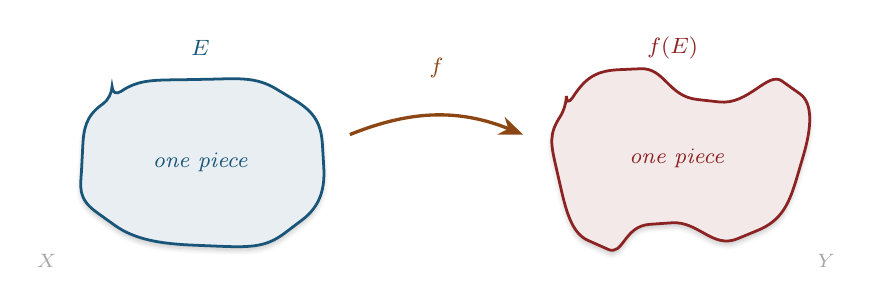
\begin{tikzpicture}[scale=1.0]
    % Domain set E (connected, one piece)
    \begin{scope}[shift={(0,0)}]
      \draw[blobblue] \blobpath;
      \node[defcolor, font=\footnotesize\itshape] at (0,0) {one piece};
    \end{scope}
    \node[defcolor, font=\footnotesize] at (0,1.45) {$E$};
    \node[gray!70, font=\scriptsize] at (-1.95,-1.25) {$X$};
    % Codomain image f(E) (connected, one piece) -- deformed, different shape
    \begin{scope}[shift={(6,0)}]
      \draw[blobred] \blobpathdef;
      \node[thmcolor, font=\footnotesize\itshape] at (0.05,0.05) {one piece};
    \end{scope}
    \node[thmcolor, font=\footnotesize] at (6,1.45) {$f(E)$};
    \node[gray!70, font=\scriptsize] at (7.95,-1.25) {$Y$};
    % curved mapping arrow
    \draw[mapf] (1.9,0.35) to[bend left=22] (4.1,0.35);
    \node[mAccent, font=\footnotesize] at (3.0,1.2) {$f$};
  \end{tikzpicture}
  \end{center}

  \note{
    Here is the central theorem of the section. Take any continuous map "f"
    from a metric space "X" into a metric space "Y". If a subset "E" of the
    domain is connected, then its image "f" of "E" is also connected. The
    picture captures the idea at a glance. On the left, in blue, sits the
    connected set "E", drawn as a single unbroken blob inside "X". The orange
    arrow is the continuous map "f". On the right, in red, is the image inside
    "Y". Notice that its outline is drawn quite differently from "E", and that
    is on purpose: a continuous map is free to stretch, bend, or squash a set
    in almost any way. The one thing it can never do is rip a connected set
    into separate pieces. So no matter how badly the shape is distorted, the
    image stays in one piece. That single idea, that continuity never tears a
    set apart, is the whole content of the theorem. Let's prove it.
  }
\end{frame}

\begin{frame}{Proof Strategy: Theorem 4.22}
  \begin{hlbox}
  \textbf{Technique:} proof by contradiction.

  \vspace{0.6em}
  \begin{enumerate}
    \item Suppose $f(E)$ \emph{is} split: $f(E) = A \cup B$, separated and nonempty.
    \item \alert{Pull back} the split to the domain: $G, H \subset E$.
    \item Show $G$ and $H$ are nonempty with $E = G \cup H$.
    \item Use continuity to show $G$ and $H$ are \alert{separated}.
    \item This contradicts $E$ being connected. \quad$\Rightarrow\Leftarrow$
  \end{enumerate}
  \end{hlbox}

  \note{
    Before the formal argument, here is the road map. We argue by
    contradiction. We start by assuming the conclusion fails, so the image
    "f" of "E" can be broken into two nonempty separated pieces, call them
    "A" and "B". The key move is to pull this break back through "f" to the
    domain, producing two pieces "G" and "H" of "E". We then check that "G"
    and "H" together make up all of "E" and that neither is empty. The heart
    of the proof is using continuity to show "G" and "H" are themselves
    separated. But that would break "E" into two separated pieces,
    contradicting the assumption that "E" is connected. Let's walk through
    each step.
  }
\end{frame}

% --- Proof step 1 ---
\begin{frame}{Proof of 4.22 --- Step 1: Assume a Split}
  \begin{proofblock}{Step 1: Suppose the image is disconnected}
    Assume $f(E) = A \cup B$, where $A, B$ are nonempty \alert{separated}
    subsets of $Y$.
    \[
      G = E \cap f^{-1}(A), \qquad H = E \cap f^{-1}(B).
    \]
  \end{proofblock}

  \vspace{0.3em}
  \begin{hlbox}
  \textbf{Idea:} $G$ is the part of $E$ landing in $A$; $H$ the part landing in $B$.
  \end{hlbox}

  \begin{center}
  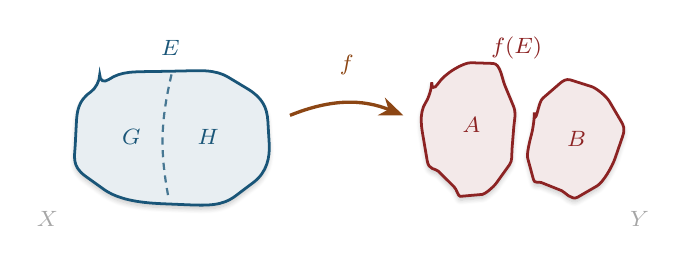
\begin{tikzpicture}[scale=0.8, every node/.style={font=\footnotesize}]
    % --- Source set E (same shape as in Theorem 4.22), split into G | H ---
    \begin{scope}[shift={(0,0)}]
      \draw[blobblue] \blobpath;
      \draw[dash pattern=on 2.6pt off 2pt, line width=0.8pt, defcolor!80]
        (0.02,1.0) to[bend right=12] (-0.02,-1.0);
      \node[defcolor] at (-0.62,0) {$G$};
      \node[defcolor] at (0.6,0) {$H$};
    \end{scope}
    \node[defcolor] at (0,1.42) {$E$};
    \node[gray!70] at (-1.95,-1.3) {$X$};
    % --- Image f(E): same deformed shape as in Theorem, now SPLIT into A and B ---
    \begin{scope}[shift={(5.5,0)}]
      % A: left piece of the deformed silhouette
      \draw[blobred]
        plot[smooth cycle, tension=0.85] coordinates
        {(-1.45,-0.2) (-1.35,0.7) (-0.55,1.18) (-0.12,0.66) (-0.06,0.0)
         (-0.22,-0.58) (-0.72,-0.92) (-1.12,-0.66)};
      % B: right piece of the deformed silhouette (gap = separation)
      \draw[blobred]
        plot[smooth cycle, tension=0.85] coordinates
        {(0.22,-0.5) (0.28,0.22) (0.55,0.74) (1.02,0.86) (1.56,0.42)
         (1.62,-0.16) (1.12,-0.86) (0.55,-0.78)};
      \node[thmcolor] at (-0.72,0.2) {$A$};
      \node[thmcolor] at (0.95,-0.02) {$B$};
    \end{scope}
    \node[thmcolor] at (5.5,1.42) {$f(E)$};
    \node[gray!70] at (7.45,-1.3) {$Y$};
    % mapping arrow
    \draw[mapf] (1.9,0.35) to[bend left=22] (3.7,0.35);
    \node[mAccent] at (2.8,1.15) {$f$};
  \end{tikzpicture}
  \end{center}

  \note{
    Step one. Suppose, for contradiction, that the image is not connected.
    Then we can write "f" of "E" as a union of two nonempty separated sets
    "A" and "B" living in "Y". In the picture, on the right is the image "f"
    of "E", the same deformed shape from the previous slide, but now broken
    into two red pieces that stay apart, "A" and "B". Now we pull this
    decomposition back into the domain, the blue set "E" on the left. Define
    "G" to be the points of "E" that "f" sends into "A", and "H" to be the
    points of "E" that "f" sends into "B"; the dashed line inside "E" marks
    this division. In symbols, "G" is "E" intersected with the preimage of
    "A", and "H" is "E" intersected with the preimage of "B". The orange
    arrow is the map "f" carrying "G" to "A" and "H" to "B". Next we check
    these pieces behave well.
  }
\end{frame}

% --- Proof step 2 ---
\begin{frame}{Proof of 4.22 --- Step 2: They Cover $E$}
  \begin{proofblock}{Step 2: $E = G \cup H$, both nonempty}
    Since $f(E) = A \cup B$, every point of $E$ maps into $A$ or $B$:
    \[
      E = G \cup H .
    \]
    As $A, B$ are nonempty, so are $G$ and $H$.
  \end{proofblock}

  \note{
    Step two. Because every value of "f" on "E" lands in either "A" or "B",
    every point of "E" belongs to "G" or to "H". So "E" is the union of "G"
    and "H". And since "A" and "B" are each nonempty, and they are both
    actually attained as images of points of "E", the pullback sets "G" and
    "H" are nonempty as well. So we have genuinely split "E" into two
    nonempty pieces. The only thing left to check, and it is the crucial
    thing, is that these two pieces are separated.
  }
\end{frame}

% --- Proof step 3 ---
\begin{frame}{Proof of 4.22 --- Step 3: Continuity Closes $G$ Down}
  \begin{proofblock}{Step 3: $f(\bar{G}) \subset \bar{A}$}
    $A \subset \bar{A} \;\Rightarrow\; G \subset f^{-1}(\bar{A})$.
    Since $f$ is continuous and $\bar{A}$ is closed, $f^{-1}(\bar{A})$ is
    \alert{closed}, so
    \[
      \bar{G} \subset f^{-1}(\bar{A}) \quad\Longrightarrow\quad f(\bar{G}) \subset \bar{A}.
    \]
  \end{proofblock}

  \note{
    Step three is where continuity does its work. Start with the obvious
    fact that "A" is contained in its closure. Taking preimages, "G" is
    contained in the preimage of the closure of "A". Now here is the key
    point: the closure of "A" is a closed set, and the preimage of a closed
    set under a continuous map is closed. We proved that characterization of
    continuity earlier in the chapter. So the preimage of the closure of "A"
    is a closed set containing "G". Therefore it must also contain the
    closure of "G", since the closure is the smallest closed set containing
    "G". Applying "f", we conclude that "f" of the closure of "G" sits inside
    the closure of "A". Let's use this.
  }
\end{frame}

% --- Proof step 4 ---
\begin{frame}{Proof of 4.22 --- Step 4: $\bar{G}$ and $H$ Don't Touch}
  \begin{proofblock}{Step 4: $\bar{G} \cap H = \varnothing$}
    $f(H) = B$ and $\bar{A} \cap B = \varnothing$. Since
    $f(\bar{G}) \subset \bar{A}$:
    \[
      \bar{G} \cap H = \varnothing .
    \]
    By symmetry, $G \cap \bar{H} = \varnothing$ as well.
  \end{proofblock}

  \vspace{0.4em}
  \hl{Hence $G$ and $H$ are \alert{separated}.}

  \note{
    Step four. Recall that "f" maps "H" onto "B", and that "A" and "B" were
    separated, so the closure of "A" does not meet "B". Now suppose a point
    lived in both the closure of "G" and in "H". Its image would lie in the
    closure of "A", from the previous step, and also in "B", because it is in
    "H". But the closure of "A" and "B" are disjoint, so that is impossible.
    Therefore the closure of "G" and "H" share no points. Running the exact
    same argument with the roles swapped shows "G" and the closure of "H"
    are also disjoint. By definition, that means "G" and "H" are separated.
  }
\end{frame}

% --- Proof conclusion ---
\begin{frame}{Proof of 4.22 --- Conclusion}
  \begin{proofblock}{Contradiction}
    $E = G \cup H$, with $G, H$ nonempty and \alert{separated}.
    \[
      \boxed{\text{This is impossible if } E \text{ is connected.}}
    \]
  \end{proofblock}

  \vspace{0.4em}
  \hl{So no such split $A \cup B$ exists: $f(E)$ is connected.} \hfill$\blacksquare$

  \note{
    And now we collect the contradiction. We have written "E" as the union
    of two nonempty separated sets "G" and "H". But that is precisely what
    cannot happen for a connected set. Since we assumed "E" is connected, our
    starting assumption, that the image could be split into separated pieces
    "A" and "B", must have been false. Therefore "f" of "E" admits no such
    split; it is connected. That completes the proof. Notice how little we
    used: only that preimages of closed sets are closed. Now let's cash this
    in for the Intermediate Value Theorem.
  }
\end{frame}
}

{
\usebackgroundtemplate{%
  
\includegraphics[width=\paperwidth,height=\paperheight,keepaspectratio=false]{chapter_04_bg_03.png}%
}
% =============================================================================
\section{The Intermediate Value Theorem}
% =============================================================================

\begin{frame}{Theorem 4.23: Intermediate Value Theorem}
  \begin{thmblock}{Theorem 4.23}
    Let $f$ be a continuous real function on $[a, b]$. If $f(a) < f(b)$ and
    $f(a) < c < f(b)$, then there exists $x \in (a, b)$ with
    $\boxed{f(x) = c}$.
  \end{thmblock}

  \vspace{0.4em}
  \begin{hlbox}
  A continuous real function on an interval \alert{assumes every
  intermediate value}. (Same conclusion if $f(a) > f(b)$.)
  \end{hlbox}

  \note{
    Here is the famous consequence. Let "f" be a continuous real valued
    function on a closed interval from "a" to "b". Suppose the value at "a"
    is less than the value at "b", and pick any number "c" strictly between
    those two values. Then the theorem guarantees there is some point "x"
    inside the open interval where "f" of "x" equals "c". In plain words, a
    continuous function on an interval cannot skip any value between two of
    its values; it assumes every intermediate value. Of course the same
    holds if the function is larger at "a" than at "b"; just reverse the
    inequality. Let's see the picture, and then how cheaply this follows
    from Theorem 4.22.
  }
\end{frame}

\begin{frame}{Intermediate Value Theorem --- Picture}
  \begin{center}
  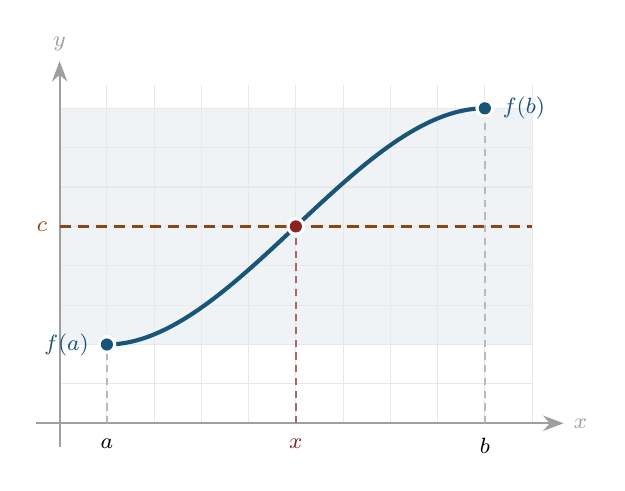
\begin{tikzpicture}[scale=1.0, font=\footnotesize]
    % Curve: x = 0.6 + 4.8t, y = 1 + 3*smoothstep(t); f(a)=1, f(b)=4, crossing (3.0,2.5)
    % faint band of attained values [f(a), f(b)]
    \fill[defcolor!7] (0,1) rectangle (6.0,4);
    % faint grid
    \draw[gray!18, line width=0.4pt, ystep=0.5, xstep=0.6] (0,0) grid (6.0,4.3);
    % axes
    \draw[axisln] (-0.3,0) -- (6.4,0) node[right, gray!75]{$x$};
    \draw[axisln] (0,-0.3) -- (0,4.6) node[above, gray!75]{$y$};
    % level c
    \draw[mapf, -, line width=1pt, dash pattern=on 4pt off 2.5pt] (0,2.5) -- (6.0,2.5);
    \node[mAccent, left=1pt] at (0,2.5) {$c$};
    % the curve
    \draw[curveln, defcolor] plot[smooth, domain=0:1, samples=100]
      ({0.6 + 4.8*\x},{1 + 3*(3*\x*\x - 2*\x*\x*\x)});
    % projection lines
    \draw[projln, gray!55] (0.6,0) -- (0.6,1);
    \draw[projln, gray!55] (5.4,0) -- (5.4,4);
    \draw[projln, thmcolor!70] (3.0,0) -- (3.0,2.5);
    % endpoint markers + labels
    \dotpt{defcolor}{(0.6,1)}
    \node[defcolor, left=3pt] at (0.6,1) {$f(a)$};
    \dotpt{defcolor}{(5.4,4)}
    \node[defcolor, right=3pt] at (5.4,4) {$f(b)$};
    % crossing point (exact)
    \dotpt{thmcolor}{(3.0,2.5)}
    % x-axis labels
    \node[below=2pt] at (0.6,0) {$a$};
    \node[below=2pt] at (5.4,0) {$b$};
    \node[thmcolor, below=2pt] at (3.0,0) {$x$};
  \end{tikzpicture}
  \end{center}

  \note{
    Let's read the diagram. The blue curve is the graph of our continuous
    function "f" over the interval from "a" to "b". On the left it starts at
    the height "f" of "a", and on the right it ends at the higher height "f"
    of "b". The horizontal orange line marks the target level "c", chosen
    somewhere between those two heights. Because the curve begins below the
    orange line and ends above it, and because it is unbroken, it has to
    cross the line somewhere. That crossing is the red dot, sitting above the
    point "x" on the axis, where "f" of "x" equals "c". The function might
    wiggle and cross several times, but the theorem only promises at least
    one crossing. Now the proof.
  }
\end{frame}

\begin{frame}{Proof of 4.23: Two Appeals to Theorem 2.47}
  \begin{proofblock}{Proof}
    \begin{enumerate}
      \item By \alert{Theorem 2.47}, $[a, b]$ is connected.
      \item By \alert{Theorem 4.22}, $f([a, b])$ is a connected subset of $R^1$.
      \item By \alert{Theorem 2.47} again, $f([a,b])$ has the \emph{in-between
            property}; as it contains $f(a), f(b)$, it contains every $c$ with
            $f(a) < c < f(b)$.
    \end{enumerate}
  \end{proofblock}

  \begin{remblock}{Recall: Theorem 2.47}
    $E \subset R^1$ is connected $\iff$ if $x, y \in E$ and $x < z < y$, then
    $z \in E$.
  \end{remblock}

  \note{
    The proof is remarkably short, and it sandwiches our new theorem between
    two uses of a Chapter 2 result. Step one: by Theorem 2.47, the closed
    interval from "a" to "b" is connected. Step two: feed that connected
    interval through our continuous function and apply Theorem 4.22, which we
    just proved; the image is a connected subset of the real line. Step
    three: apply Theorem 2.47 in the other direction. It says a connected set
    on the line has no gaps: whenever it contains two points, it contains
    every point between them. One subtle point worth stressing, shown in the
    gray box: this does not force the set to be a closed interval. The
    boundary points may or may not belong to it, so the image could be open,
    half open, or closed. That does not matter here, though, because all we
    need is that the image contains "f" of "a" and "f" of "b", and therefore
    every value "c" strictly between them. So some point maps to "c". Done.
  }
\end{frame}
}

{
\usebackgroundtemplate{%
  
\includegraphics[width=\paperwidth,height=\paperheight,keepaspectratio=false]{chapter_04_bg_04.png}%
}
% =============================================================================
\section{Is There a Converse?}
% =============================================================================

% --- Build 1/2 ---
\begin{frame}{Remark 4.24: A Tempting Converse}
  \begin{remblock}{Remark 4.24: does the converse hold?}
    One might guess: if $f$ takes every intermediate value on every
    subinterval, must $f$ be \alert{continuous}?
  \end{remblock}

  \vspace{0.5em}
  \begin{hlbox}
  More precisely: for all $x_1 < x_2$ and every $c$ between $f(x_1)$ and
  $f(x_2)$, there is $x \in (x_1, x_2)$ with $f(x) = c$.
  \end{hlbox}

  \note{
    Here is a natural and tempting question. The Intermediate Value Theorem
    says continuity implies the intermediate value property. Does the arrow
    run the other way? That is, suppose a function "f" has the intermediate
    value property on every subinterval: for any two points "x" one and "x"
    two, and any "c" between the corresponding values, the function actually
    hits "c" somewhere in between. It feels like such a function should be
    forced to be continuous, since it never seems to skip a value. Let's see
    whether that intuition holds up.
  }
\end{frame}

% --- Build 2/2 ---
\begin{frame}{Remark 4.24: The Converse Is False}
  \begin{remblock}{Remark 4.24: does the converse hold?}
    One might guess: if $f$ takes every intermediate value on every
    subinterval, must $f$ be \alert{continuous}?
  \end{remblock}

  \vspace{0.3em}
  \begin{center}
  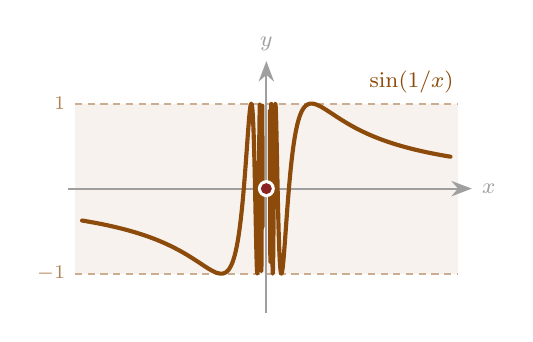
\begin{tikzpicture}[scale=0.9, font=\footnotesize]
    % amplitude band where the oscillation lives
    \fill[excolor!7] (-2.7,-1.2) rectangle (2.7,1.2);
    \draw[projln, excolor!45] (-2.7,1.2) -- (2.7,1.2);
    \draw[projln, excolor!45] (-2.7,-1.2) -- (2.7,-1.2);
    \node[excolor!70, font=\scriptsize, left] at (-2.7,1.2) {$1$};
    \node[excolor!70, font=\scriptsize, left] at (-2.7,-1.2) {$-1$};
    % axes
    \draw[axisln] (-2.8,0) -- (2.9,0) node[right, gray!75]{$x$};
    \draw[axisln] (0,-1.75) -- (0,1.8) node[above, gray!75]{$y$};
    % y = sin(1/x); the "r" suffix marks the argument as radians
    \draw[curveln, excolor] plot[smooth, domain=0.05:2.6, samples=500]
      ({\x},{1.2*sin((1/\x) r)});
    \draw[curveln, excolor] plot[smooth, domain=-2.6:-0.05, samples=500]
      ({\x},{1.2*sin((1/\x) r)});
    % value assigned at the origin
    \dotpt{thmcolor}{(0,0)}
    \node[excolor] at (2.05,1.5) {$\sin(1/x)$};
  \end{tikzpicture}
  \end{center}
  \begin{center}
  \hl{\alert{No.} Example 4.27($d$): $f(x) = \sin(1/x)$, $f(0) = 0$.}
  \end{center}

  \note{
    The answer is no, and the counterexample is a function we will meet
    again, Example 4.27 part "d". Define "f" of "x" to be the sine of one
    over "x" away from the origin, and zero at the origin. As the picture
    shows, near zero this function oscillates faster and faster between minus
    one and one, packing in infinitely many wiggles. Because of those
    oscillations, on any interval touching the origin the function sweeps
    through every value between minus one and one, so it does have the
    intermediate value property. Yet it is wildly discontinuous at the
    origin, since it has no limit there; the left and right hand limits
    simply do not exist. So the intermediate value property is genuinely
    weaker than continuity. The converse fails.
  }
\end{frame}
}

{
\usebackgroundtemplate{%
  
\includegraphics[width=\paperwidth,height=\paperheight,keepaspectratio=false]{chapter_04_bg_05.png}%
}
% =============================================================================
\section{Summary}
% =============================================================================

% --- Build 1/3 ---
\begin{frame}{Summary}
  \begin{hlbox}
  \textbf{Key takeaways:}
  \begin{itemize}
    \item \alert{Theorem 4.22:} continuity preserves \emph{connectedness} ---
          $f(E)$ is connected whenever $E$ is.
  \end{itemize}
  \end{hlbox}

  \note{
    Let's gather what we learned. The first and central result is Theorem
    4.22: a continuous map carries connected sets to connected sets. Just as
    continuity preserved compactness in the previous section, it preserves
    connectedness here. The proof was a clean contradiction argument, pulling
    a hypothetical split of the image back to the domain and using only the
    fact that preimages of closed sets are closed.
  }
\end{frame}

% --- Build 2/3 ---
\begin{frame}{Summary}
  \begin{hlbox}
  \textbf{Key takeaways:}
  \begin{itemize}
    \item \alert{Theorem 4.22:} continuity preserves \emph{connectedness} ---
          $f(E)$ is connected whenever $E$ is.
    \item \alert{Theorem 4.23:} the \emph{Intermediate Value Theorem} ---
          a continuous function on $[a,b]$ hits every value between $f(a)$ and $f(b)$.
  \end{itemize}
  \end{hlbox}

  \note{
    The second takeaway is the celebrated payoff: the Intermediate Value
    Theorem. A continuous real function on a closed interval takes on every
    value between its endpoint values. And the proof was almost free: sandwich
    Theorem 4.22 between two applications of the Chapter 2 fact that connected
    subsets of the line are exactly the intervals. This is a beautiful example
    of how a general topological theorem yields a concrete classical result.
  }
\end{frame}

% --- Build 3/3 ---
\begin{frame}{Summary}
  \begin{hlbox}
  \textbf{Key takeaways:}
  \begin{itemize}
    \item \alert{Theorem 4.22:} continuity preserves \emph{connectedness} ---
          $f(E)$ is connected whenever $E$ is.
    \item \alert{Theorem 4.23:} the \emph{Intermediate Value Theorem} ---
          a continuous function on $[a,b]$ hits every value between $f(a)$ and $f(b)$.
    \item \alert{Remark 4.24:} the converse \emph{fails} --- the intermediate
          value property does not imply continuity ($\sin(1/x)$).
  \end{itemize}
  \end{hlbox}

  \vspace{0.6em}
  \begin{hlbox}
  \textbf{Coming up next:} \emph{Discontinuities} --- classifying the ways
  continuity can break down.
  \end{hlbox}

  \note{
    The third takeaway is a cautionary one. It is tempting to believe the
    Intermediate Value Theorem has a converse, that the intermediate value
    property forces continuity. But it does not. The function sine of one
    over "x" has the intermediate value property near the origin yet is badly
    discontinuous there. So continuity is strictly stronger. That naturally
    leads into our next section, on discontinuities, where we classify the
    different ways a function can fail to be continuous. Thanks for watching,
    and see you in the next section.
  }
\end{frame}
}

\end{document}
